
\documentclass[11pt,a4paper]{article}
\usepackage[utf8]{inputenc}
\usepackage[T1]{fontenc}
\usepackage{lmodern}
\usepackage[margin=2.35cm]{geometry}
\usepackage{microtype}
\usepackage{graphicx}
\usepackage{booktabs}
\usepackage{longtable}
\usepackage{tabularx}
\usepackage{array}
\usepackage{float}
\usepackage{fancyhdr}
\usepackage{xcolor}
\usepackage{hyperref}
\usepackage{enumitem}
\usepackage{setspace}
\usepackage{caption}
\usepackage{titlesec}
\usepackage{amsmath}
\usepackage{ragged2e}
\usepackage{etoolbox}
\usepackage{multicol}
\usepackage{lastpage}

\definecolor{accent}{HTML}{163A5F}
\definecolor{softline}{HTML}{D7E2EE}
\definecolor{textgray}{HTML}{4A5560}
\definecolor{boxfill}{HTML}{F4F8FC}
\definecolor{lightaccent}{HTML}{EAF1F8}

\hypersetup{
  colorlinks=true,
  linkcolor=accent,
  citecolor=accent,
  urlcolor=accent,
  pdftitle={An Actionable Model for Proactive Detection of Fraud},
  pdfauthor={Graz Network}
}

\pagestyle{fancy}
\fancyhf{}
\fancyhead[L]{\footnotesize\color{textgray}Actionable model for proactive detection of fraud}
\fancyfoot[C]{\footnotesize\thepage\,/\pageref{LastPage}}
\renewcommand{\headrulewidth}{0.25pt}
\renewcommand{\footrulewidth}{0pt}

\setstretch{1.08}
\setlength{\parskip}{0.48em}
\setlength{\parindent}{0pt}
\setlist[itemize]{leftmargin=1.45em,itemsep=0.18em,topsep=0.18em}
\setlist[enumerate]{leftmargin=1.5em,itemsep=0.18em,topsep=0.18em}
\setcounter{tocdepth}{1}
\titleformat{\section}{\Large\bfseries\color{accent}}{\thesection}{0.6em}{}
\titleformat{\subsection}{\large\bfseries\color{accent}}{\thesubsection}{0.6em}{}
\captionsetup{font=small,labelfont=bf}
\urlstyle{same}

\newcolumntype{Y}{>{\RaggedRight\arraybackslash}X}
\newcommand{\topruleline}{\color{accent}\rule{\textwidth}{1.2pt}}
\newcommand{\midruleline}{\color{accent}\rule{\textwidth}{0.7pt}}
\newcommand{\callout}[1]{%
  \noindent\fcolorbox{softline}{boxfill}{%
    \parbox{\dimexpr\linewidth-2\fboxsep-2\fboxrule\relax}{#1}}
}

\begin{document}
\thispagestyle{empty}

{\topruleline}
\begin{center}
{\LARGE\bfseries An Actionable Model for Proactive Detection of Fraud:}\\[0.2em]
{\LARGE\bfseries A Transparent, Auditable Method for Higher-Risk Online Listings}\\[0.65em]
{\large Graz Network}\\[0.8em]
{\small March 2026}
\end{center}
{\topruleline}

\section*{Abstract}
This article reworks the MASLCE thesis \emph{\`Elaboration d'un modele actionnable pour la detection proactive des petites annonces frauduleuses} into a publication-oriented English paper addressed to professionals concerned with economic crime, cybercrime, online-marketplace abuse, and digital-risk governance. The original study asked a practical question: how can fraudulent listings be detected efficiently and reliably \emph{before} additional victims are harmed? To answer that question, the project combined an exploratory qualitative phase with a quantitative validation phase. Six exploratory interviews involving nine cybercrime practitioners were used to convert field knowledge into a compact three-indicator model built around price anomaly, content similarity or duplication, and profile recency. These indicators were transformed into an additive risk index and then into an operational target contrasting \emph{acceptable} and \emph{unfavorable} fraud risk. Reproduction from the archived project corpus confirms the internal coherence of the main case-study result on the canonical sample of 2,166 Facebook Marketplace listings: accuracy 0.954, precision 0.940, recall 0.975, specificity 0.930, and AUC 0.978. At the same time, a full evaluation shows why the model must be interpreted carefully. The broader target remains an internal risk label rather than a direct repository of judicially proven fraud; the evidence base is platform-specific and product-heavy; and the archive required canonicalisation because multiple file versions coexist. On that basis, the article argues that the research is publication-ready not as a universal fraud-classification benchmark, but as a strong contribution to proactive fraud triage. Its real value is to offer a transparent, auditable, and operationally meaningful method for identifying higher-risk listings in a context where purely reactive enforcement remains insufficient.

\textbf{Keywords:} fraud detection; online classified ads; proactive screening; cybercrime; economic crime; actionable knowledge; auditability; risk triage

\newpage

\tableofcontents

\newpage

\section{Introduction}
Fraudulent online listings are a classic example of a low-individual-loss but high-volume crime problem. A single deceptive listing may generate a relatively modest loss, yet the phenomenon becomes strategically important because the model scales, replicates quickly, exploits routine digital commerce, and frequently remains below the threshold of strong institutional reaction. The MASLCE thesis developed by David Graz began from exactly that operational tension. In the ratified project design, the research question was framed in plain and practice-oriented terms: how can fraudulent small ads be detected efficiently and reliably? The underlying concern was not merely academic description. It was the persistent difficulty of acting \emph{before} victim complaints accumulate, evidence disappears, and the most useful traces have already been lost.

That starting point remains highly relevant for professionals engaged in the fight against economic crime and cybercrime. In online-classified environments, the window for intervention is short. A listing can be created, duplicated, shared, taken down, and recreated elsewhere before any reactive chain becomes effective. When institutions rely primarily on victim reporting, the practical sequence is often unfavourable: a loss occurs, the listing disappears, the communication trail is partial, the platform data are limited, and any later attempt at attribution becomes more costly. In this setting, the value of a proactive method is not that it ends uncertainty. The value is that it improves triage and action while uncertainty still remains manageable.

The thesis approached this problem through an actionable-knowledge perspective. Rather than beginning with a technically ambitious but opaque machine-learning architecture, it asked which recurrent signs practitioners already use when they suspect a listing is deceptive. Across the qualitative material, three themes stabilised into operational indicators: implausibly low prices, repetitive or duplicated content, and recent or weakly documented seller profiles. These indicators were formalised into scores, summed into an index, and later used in a predictive model. The resulting system is therefore better understood as an operational language of risk than as a universal theory of digital fraud.

This distinction matters. Many fraud-detection papers emphasise predictive lift, model architecture, or benchmark comparison. The MASLCE project is different. Its strongest contribution lies in the conversion of dispersed professional know-how into a compact, intelligible, and auditable framework that can be deployed for early screening. That is why the most defensible reading of the research is also the most useful one: the work does not establish a self-sufficient proof engine, but a transparent method for identifying higher-risk listings in an environment where reactive enforcement alone is structurally insufficient.

This article has four aims. First, it transforms the thesis into a standard academic article in English. Second, it explains the research process in a form suitable for publication-jury review. Third, it evaluates the integrity of the research basis using the documented reconstruction work already completed in this project. Fourth, it draws out the study's main practical contribution for economic-crime and cybercrime professionals. The central argument is straightforward: when interpreted as a proactive fraud-triage model rather than as universal adjudicative truth, the MASLCE research is strong, publishable, and operationally relevant.

\section{Why reactive enforcement is not enough}
Reactive enforcement remains indispensable, but the research underlying this article shows why it struggles when confronted with fraudulent listing ecosystems. The first difficulty is scale. Fraudulent ads do not need to be individually sophisticated in order to be harmful at system level. They only need to be good enough, numerous enough, and persistent enough to recruit responses from a fraction of the audience. This dynamic is well known in scam literature and appears again in the MASLCE corpus: the real power of the phenomenon lies in repetition, not in singular brilliance.

The second difficulty is attrition of evidence. In the thesis interviews, practitioners repeatedly described the same operational problem: when victims finally report, the listing has often been deleted, the seller profile has changed, and the original exchange is incomplete. The trace value of the event has already degraded. This does not make investigation impossible, but it shifts the case toward a more expensive and less reliable mode of reconstruction. By contrast, proactive detection preserves optionality. Even if a suspicious listing is not immediately attributable, an early flag can trigger evidence-preserving action, platform notification, or enhanced monitoring.

The third difficulty is organisational fragmentation. Digital marketplaces do not sit under a simple police monopoly. Platforms, private trust-and-safety units, regulators, users, consumer-protection actors, and police services all possess fragments of the security function. The MASLCE project correctly treats this environment as ecosystemic rather than unitary. In such a setting, a good detection model must do more than generate a score. It must create a shared language that can move across institutions with different mandates and different evidentiary thresholds.

The fourth difficulty is the mismatch between legal finality and operational necessity. Professionals often need to decide under conditions of incomplete information. A platform moderator deciding whether to prioritise review, an intelligence analyst deciding whether to preserve traces, and a prevention officer deciding whether to issue a warning do not all need the same epistemic threshold as a court. This is the practical space into which the MASLCE model fits. It offers a reasoned basis for graded action before final legal determination is available.

Finally, the thesis and the associated reconstruction also show why the problem is likely to persist. Fraudulent small ads borrow from longstanding scam logics while adapting to contemporary platforms. The medium changes faster than the basic manipulative mechanisms. That combination makes a purely reactive posture chronically vulnerable. The study's main policy implication therefore begins here: proactive detection is not a luxury add-on to casework. In high-volume fraud environments, it is a necessary complement to reactive enforcement.

\section{Research basis and article framing}
This article rests on a layered documentary basis preserved in the MASLCE project corpus. The ratification form defined the original problem, theoretical orientation, and intended mixed-method design. The completed thesis reported the final methodology, indicator model, quantitative results, discussion, and bibliography. The defence slides condensed the project's operational interpretation and headline findings. The wider archive contained datasets, scripts, thematic notes, and supporting materials. In the documented reconstruction already completed for this project, these materials were reviewed, sanitised, and canonicalised so that the quantitative claims could be reproduced in a controlled way.

That reconstruction matters because the archive is rich but not version-clean. It contains multiple copies, drafts, and legacy scripts. A publication-grade article cannot simply assume that every file has equal evidentiary status. The present article therefore relies on the canonical samples and on reproduced metrics rather than on unreviewed archival multiplicity. This approach strengthens, rather than weakens, the article. It makes the reasoning explicit, separates stable claims from unstable artefacts, and keeps the final publication aligned with what can actually be documented.

The article's framing follows the strongest defensible interpretation of the research. The model is presented as a proactive risk-triage instrument that helps identify higher-risk listings. It is \emph{not} framed as a universal fraud classifier; it is \emph{not} presented as a substitute for judicial proof; and it is \emph{not} claimed to be externally validated across platforms, product categories, or national settings. Those boundaries are central to its credibility. On those terms, however, the research is strong enough for publication-jury examination.

\section{Conceptual foundations of the model}
\subsection{Actionable knowledge}
The first foundation of the MASLCE project is the actionable-knowledge framework associated with Avenier and Schmitt \cite{avenier2007a,avenier2007b}. Their work is important here because it shifts the value criterion of research. Knowledge is not judged only by descriptive elegance or theoretical abstraction; it is also judged by whether it can guide action in complex organisational settings. This is especially relevant in fraud environments where practitioners often possess strong intuitions but weak formalisation. Investigators may know that certain listings feel wrong, yet that tacit judgement is difficult to explain, transmit, audit, or calibrate.

The thesis responds directly to that problem. It turns scattered observations into a small set of indicators that can be scored, compared, communicated, and revised. This is one reason the study is more interesting than a generic benchmark exercise. It offers a model of how professional intuition can be disciplined into an operational framework without being replaced by a black box.

\subsection{Trace and indicia reasoning}
The second foundation is Ribaux's indicia methodology \cite{ribaux2023}. Within this perspective, a listing is not merely content; it is a digital trace produced by an action sequence. That trace can be examined for signs that are individually incomplete but collectively informative. The asking price, the wording of the description, the pattern of duplication, and the age of the profile do not by themselves establish criminal intent. Yet together they can shift the probability landscape enough to justify preventive action.

This is a major conceptual strength. It protects the study from the false choice between naive certainty and total scepticism. The model does not claim to know everything from one signal. It claims that a limited set of recurring signals can form a meaningful basis for graded suspicion. For practitioners, that is exactly the right level of ambition.

\subsection{Ecosystemic cybercrime governance}
The third foundation is Dupont's ecosystemic interpretation of cybercrime \cite{dupont2014,dupont2024}. Fraudulent online listings emerge in a fragmented environment where commercial incentives, platform design, law-enforcement capacity, private moderation, and user behaviour interact. From this viewpoint, the utility of the MASLCE model is not confined to a single institutional actor. A platform can use it for queue prioritisation, a prevention officer can use it for warning design, and an analyst can use it for risk-graded review. The same indicators can thus support coordination across actors that do not share the same mandate or threshold of proof.

\subsection{Literature on fraud indicators and detection}
The thesis bibliography places the project within a broader body of work on online-classified fraud, deceptive advertising, phishing-like redirection, money-mule recruitment, and machine-assisted anomaly detection \cite{alrousan2020,alzghoul2024,mccormick2013,shaukat2023,saumya2022,nanath2023,leukfeldt2017,mokhberi2024}. This literature consistently points to a cluster of red flags that overlap with the MASLCE model: unusually attractive offers, repeated or templated content, low-credibility seller identities, and evasive interaction patterns. The research contribution is therefore not the invention of entirely new indicators. It is the operational reassembly of known signs into a concise model that professionals can inspect and act on.

That distinction is important for publication positioning. Articles can be original either because they discover new variables or because they make existing knowledge operationally usable in a new way. The MASLCE project belongs to the second category. Its originality lies in operational formalisation, transparency, and transferability.

\section{Study design and research process}
\subsection{Sequential exploratory mixed methods}
At design level, the project follows a sequential exploratory mixed-method logic \cite{fortin2022,thomas2006}. A qualitative phase comes first in order to explore the phenomenon, gather practitioner knowledge, and stabilise operational categories. A quantitative phase follows in order to test whether the formalised indicators can discriminate between lower-risk and higher-risk listings on real data. This sequence is coherent with the research question. When the goal is to transform tacit knowledge into an operational tool, starting with qualitative elicitation is methodologically sound.

\subsection{Qualitative phase}
The qualitative phase relied on six exploratory interviews involving nine specialists in cybercrime-related functions across francophone Swiss policing and research settings. The project used semi-structured interviewing and thematic analysis to identify recurring problem descriptions, practical bottlenecks, and detection cues. Across the interview notes and thesis narrative, several motifs recur: fragmented responsibility for online safety, the absence of sufficiently proactive tools, the internationalisation of fraud activity, the operational value of prevention, and repeated reference to low prices, copied content, and recent profiles as practical red flags.

These interviews should not be over-generalised. The sample is small and purposive. Yet for the purposes of exploratory model building, it is fit for role. The project did not require statistical representativeness at this stage; it required informed professional perspectives capable of stabilising operational categories.

\subsection{Quantitative phase}
The quantitative phase used manually collected Facebook Marketplace data. Two canonical datasets were identified in the archive during reproduction. The first, an exploratory verification sample, contains 315 listings selected to test the theoretical model under suspicion-enriched conditions. The second, a broader case-study sample, contains 2,166 listings and functions as the main quantitative stress test.

A major practical point deserves emphasis. The data are platform-specific and product-heavy, particularly around iPhone listings. This affects external validity, but it does not nullify the study's contribution. It means the article should be read as a well-documented operational pilot rooted in one environment rather than as a universal cross-market benchmark.

\subsection{Data handling, legality, and ethics}
The thesis is attentive to legal and ethical constraints on data collection. It explicitly limits collection to public-facing information and recognises platform terms, privacy rules, and copyright issues. Manual capture was used rather than unrestricted scraping. For professionals, this feature is double-edged. On the one hand, it reduces legal risk and keeps the model close to observable public traces. On the other hand, it constrains scale and excludes richer proprietary signals that platforms themselves might use. The resulting model is therefore realistic for low-access environments but not exhaustive of what a well-instrumented platform could do.

\subsection{Operationalisation of the indicators}
The model operationalises three indicators as simple ordinal scores. Price anomaly is evaluated against benchmark market values. Content similarity uses archived similarity logic grounded in Jaccard-style thresholds. Profile recency uses the age of the account or its absence where the platform displays incomplete profile age. These components are combined into an additive index that is then thresholded into acceptable or unfavorable risk.

\begin{table}[H]
\centering
\caption{Operationalisation of the three-indicator model.}
\begin{tabularx}{\textwidth}{p{3.2cm} p{1.5cm} Y}
\toprule
\textbf{Indicator} & \textbf{Score range} & \textbf{Operational meaning} \\
\midrule
Price anomaly & 1--3 & 1 = market-consistent price; 2 = underpriced; 3 = suspiciously low. The archived model used benchmark ratios that classify offers below half the benchmark as strongly suspicious. \\
Content similarity & 1--3 & 1 = unique content; 2 = similar content; 3 = duplicated content. The archived logic relied on thresholded similarity values derived from textual overlap. \\
Profile recency & 1--3 & 1 = older profile; 2 = intermediate or missing profile age; 3 = new profile. The model treats recent or opaque profiles as operationally riskier than established ones. \\
Fraud index & 3--9 in canonical data & Additive sum of the three scores. Listings at or below the acceptance threshold are coded as \emph{acceptable} risk; those above it are coded as \emph{unfavorable} risk. \\
\bottomrule
\end{tabularx}
\end{table}

This operationalisation is one of the study's strongest design choices. Even before the predictive model is considered, the index is already understandable and auditable. An analyst can explain why a listing was flagged, a supervisor can revise thresholds, and a platform can test alternative calibration rules. That degree of visibility is unusually valuable in settings where explainability is not optional.

\subsection{Predictive modelling and documented reproduction}
The predictive phase uses a random-forest classifier with cross-validation. In itself, that modelling choice is not novel. Its value lies in demonstrating that the compact index structure carries enough signal to support practical discrimination between risk categories. The documented reconstruction carried out in this project reproduced the key metric blocks and also tested how stable the results remained after removing one undesirable variable in an exploratory script. The broader conclusion is reassuring: the model's substantive value does not collapse once the archive is cleaned, even though the archive did require version control and reporting corrections.

\section{What the qualitative phase contributed}
A practitioner-oriented reading of the qualitative phase yields three important outputs.

First, the interviews clarified the nature of the operational gap. The problem was not a total absence of professional intuition. The problem was that relevant know-how remained fragmented, difficult to standardise, and weakly convertible into a repeatable screening process. This justifies the actionable-knowledge framing.

Second, the interviews identified a small set of recurring red flags that appeared robust enough to move into formal scoring. Practitioners repeatedly referred to unrealistic prices, copied descriptions, and newly created profiles. The fact that these same signals later proved useful in the quantitative phase strengthens the mixed-method coherence of the project.

Third, the interviews situated fraud detection inside a broader ecology of responsibility. Respondents highlighted platform asymmetry, international barriers, prevention needs, and the limits of reactive casework. These observations are not secondary. They explain why a transparent triage model has value even when it falls short of definitive attribution. The model helps actors coordinate under conditions where no single institution sees the whole picture.

\section{Quantitative basis and reproduced findings}
\subsection{Canonical data basis}
The documented audit identified two canonical datasets. Table~\ref{tab:basis} summarises the principal quantitative basis used for this article.

\begin{table}[H]
\centering
\caption{Canonical quantitative basis used in the article reconstruction.}
\label{tab:basis}

\renewcommand{\arraystretch}{1.2} % better vertical spacing

\begin{tabularx}{\textwidth}{>{\raggedright\arraybackslash}p{7cm} >{\centering\arraybackslash}X >{\raggedright\arraybackslash}p{7cm}}
\toprule
\textbf{Dataset} & \textbf{Size} & \textbf{Risk split} \\
\midrule

Exploratory verification sample & 315 & 34 acceptable / 281 unfavorable \\

\addlinespace[0.3em]
\multicolumn{3}{>{\raggedright\arraybackslash}p{15cm}}{\textit{Interpretive note:} Suspicion-enriched sample used to test the theoretical model under concentrated conditions. The archive also contains 114 positive and 7 negative source-status cases at the confirmed extremes.} \\
\midrule
\addlinespace[0.8em]

Case-study sample & 2,166 & 1,015 acceptable / 1,151 unfavorable \\

\addlinespace[0.3em]
\multicolumn{3}{>{\raggedright\arraybackslash}p{15cm}}{\textit{Interpretive note:} Broader operational stress test. The canonical source-status counts include 18 positive and 343 negative extreme cases, alongside larger detected and identified groups.} \\

\bottomrule
\end{tabularx}
\end{table}

The class structure is important. The stronger metric claims in the thesis concern prediction of the internal risk target, not complete adjudication across all source-status categories. That does not make the result trivial; it means the result must be interpreted at the correct level.

\subsection{Exploratory sample}
The exploratory sample is intentionally rich in suspicious listings. Within this dataset, unfavorable risk dominates. The reproduced metrics show decent overall performance with strong recall but low specificity: accuracy 0.873, precision 0.914, recall 0.947, specificity 0.265, and AUC 0.826. In operational terms, the model does well at capturing high-risk listings in the sample, but it is much less conservative in protecting low-risk listings from false alarms.

This is not necessarily a fatal weakness, because the sample is not designed as a neutral prevalence environment. Still, it matters analytically. It shows that the model's earliest quantitative form should not be treated as publication-grade proof by itself. The exploratory phase supports plausibility, not finality.

\subsection{Case-study sample}
The case-study sample is the article's strongest quantitative base. Here the model achieves accuracy 0.954, precision 0.940, recall 0.975, specificity 0.930, and AUC 0.978 under reproduction. These values are strong enough to justify serious professional interest, especially because they arise from a compact and interpretable indicator system rather than from a highly opaque feature stack.

At the same time, the article must state what these metrics mean. They mean that the model discriminates very well between the study's internal acceptable-risk and unfavorable-risk categories. They do \emph{not} mean that every unfavorable listing is legally proven fraud. The distinction is methodologically crucial and operationally healthy.

\begin{figure}[H]
    \centering
    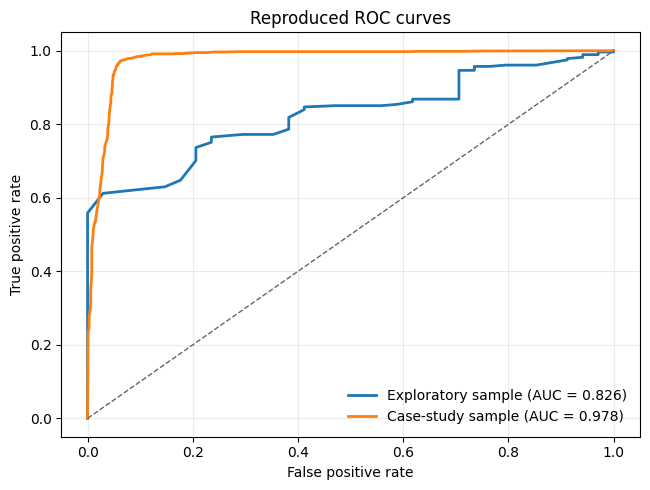
\includegraphics[width=0.96\textwidth]{../figures/roc_curves.png}
    \caption{Reproduced ROC curves for the exploratory and case-study samples. The case-study result is the article's strongest quantitative finding.}
\end{figure}

\begin{table}[H]
\centering
\caption{Reproduced predictive performance from the canonical MASLCE reconstruction.}
\begin{tabularx}{\textwidth}{p{5.1cm} c c c c c c}
\toprule
\textbf{Evaluation} & \textbf{Accuracy} & \textbf{Precision} & \textbf{Recall} & \textbf{F1} & \textbf{Specificity} & \textbf{AUC} \\
\midrule
Exploratory sample, archived script & 0.873 & 0.914 & 0.947 & 0.930 & 0.265 & 0.826 \\
Exploratory sample, clean rerun & 0.879 & 0.912 & 0.957 & 0.934 & 0.235 & 0.841 \\
Case-study sample, canonical script & 0.954 & 0.940 & 0.975 & 0.957 & 0.930 & 0.978 \\
Confirmed-extremes validation, case-study subset & 0.994 & 1.000 & 0.889 & 0.941 & 1.000 & 0.999 \\
\bottomrule
\end{tabularx}
\end{table}

\subsection{Indicator composition in the broader sample}
The reproduced case-study distributions also support the substantive relevance of the three indicators. Unfavorable-risk cases are more strongly associated with suspiciously low prices, content duplication or heavy similarity, and recent or opaque profiles than acceptable-risk cases are. Meanwhile, older profiles cluster more strongly among acceptable-risk listings.

\begin{figure}[H]
    \centering
    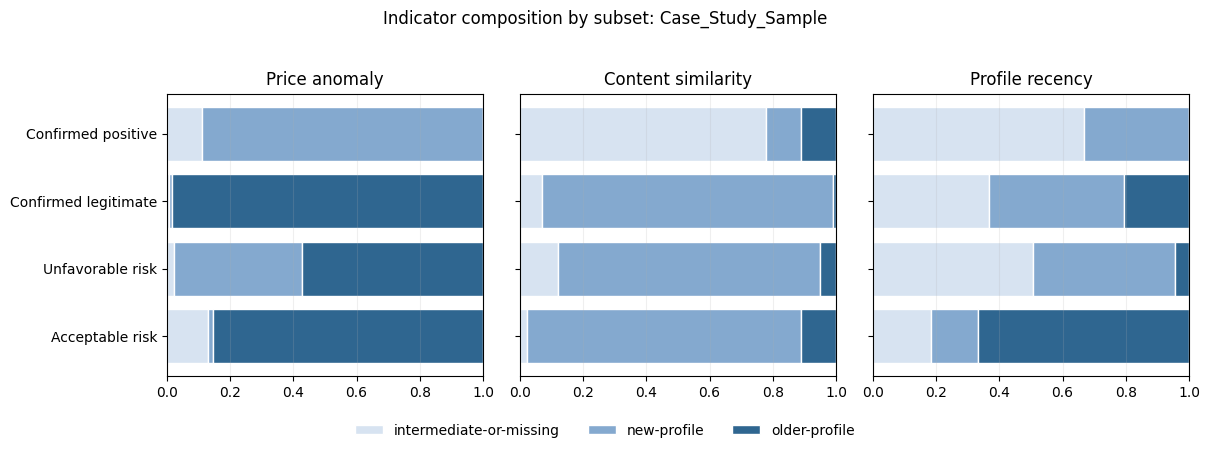
\includegraphics[width=0.98\textwidth]{../figures/case_indicator_distribution.png}
    \caption{Indicator composition across subsets in the canonical case-study sample. The manually confirmed-positive subset is small, but it concentrates heavily in the suspicious price and duplicated-content bands.}
\end{figure}

The small confirmed-positive subset in the broader sample is a limitation, but it is also informative. Among these extreme cases, duplicated content and suspicious prices are strongly overrepresented, while older profiles are absent. This pattern does not prove universality, yet it does support the model's operational logic.

\section{The model's main real contribution}
Professionals evaluating this research should focus on what the model genuinely contributes rather than on what an inflated reading might claim for it. The real contribution is not a novel machine-learning pipeline. The real contribution is the design of a transparent, auditable, operationally meaningful framework for identifying higher-risk listings early enough to support action.

That contribution has four components.

\textbf{First, the model translates field knowledge into a repeatable screen.} Investigators and analysts often rely on recurring cues, but those cues are rarely formalised in a way that supports transmission and review. The MASLCE model turns tacit suspicion into a documented scoring structure.

\textbf{Second, the model preserves a human decision point.} Because the index is interpretable, it does not force professionals into a blind trust relationship with the machine. A flagged listing can be reviewed, contextualised, and either escalated or dismissed with reasons. This is a major practical advantage where false positives carry reputational or legal consequences.

\textbf{Third, the model supports auditability.} The same score can be stored with indicator values, threshold versions, and analyst notes. This creates an audit trail that is often missing from looser preventive processes. In practice, auditability matters not only for accountability but also for learning. Professionals need to know which false positives recur, which threshold settings drift, and which new fraud patterns are not yet captured.

\textbf{Fourth, the model is operationally flexible.} It can be used for queue prioritisation, warning systems, preliminary moderation, intelligence-led monitoring, or public-private coordination. Its value does not depend on a single deployment context.

\begin{figure}[H]
    \centering
    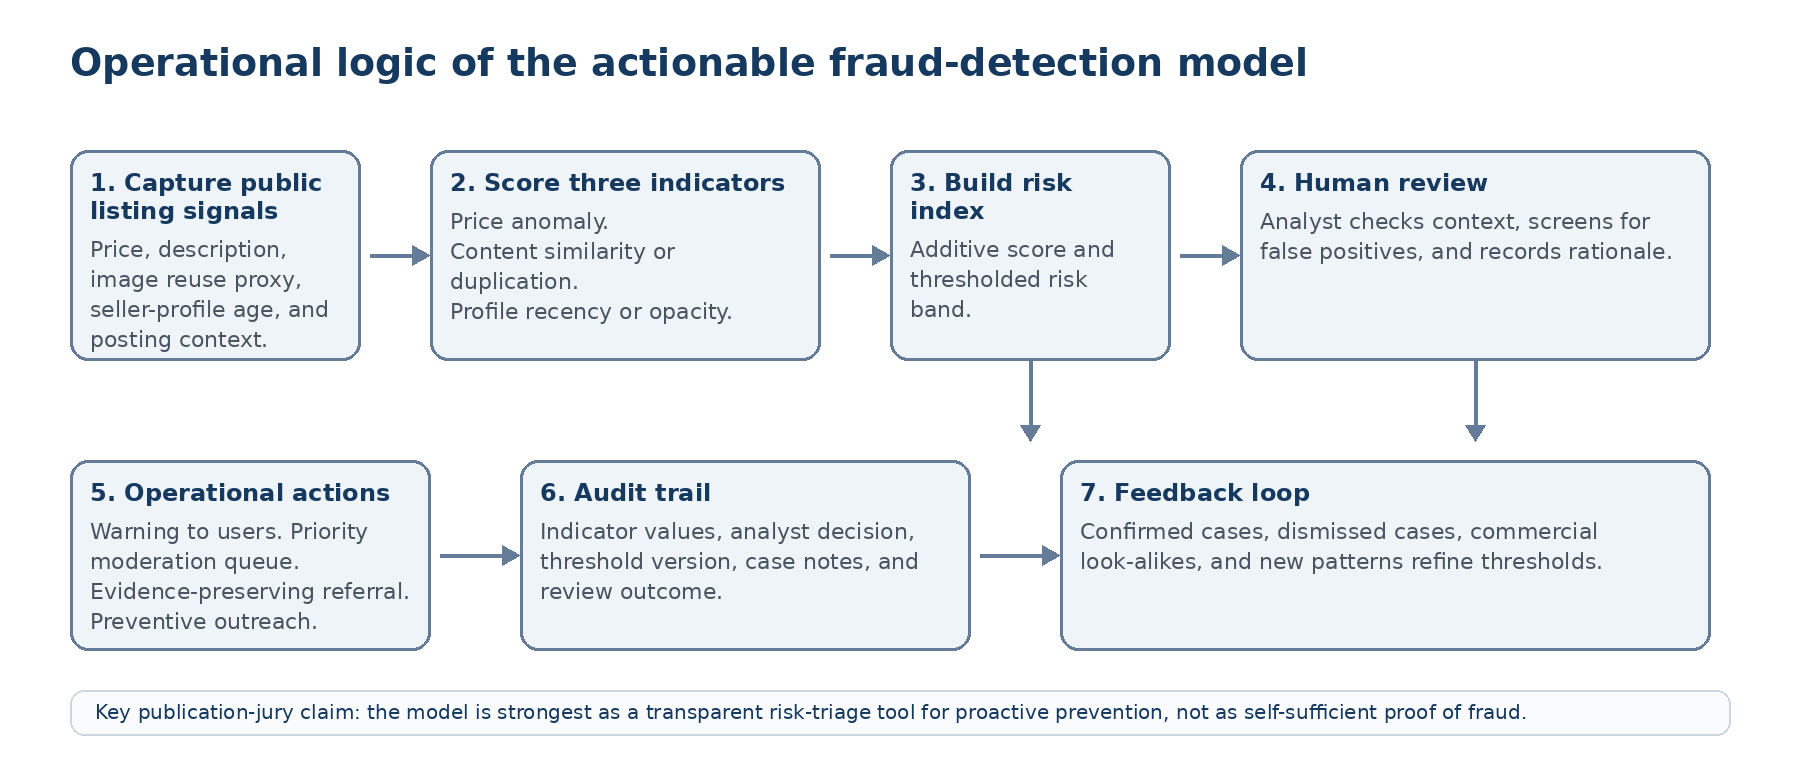
\includegraphics[width=0.96\textwidth]{../figures/operational_workflow.png}
    \caption{Operational logic of the actionable model when deployed as a risk-triage system rather than as an autonomous proof engine.}
\end{figure}

This is why the article insists on a specific formulation: the research is ready for publication-jury examination when its contribution is defined as proactive risk triage in support of prevention, moderation, evidence preservation, and early coordination. On those terms, the model is both more modest and more credible than a universal fraud-classification claim.

\section{Integrity, reproducibility, and limits}
A complete publication-jury article must state not only the study's strengths but also the integrity issues uncovered during reconstruction.

\subsection{What reproduced well}
The main descriptive totals in the canonical datasets reproduce cleanly, and the principal case-study metric block stands up well under rerun. This is important because it shows that the headline quantitative contribution is not a fragile artefact of a single broken script. The mixed-method sequence is also coherent: qualitative categories and quantitative indicators clearly align.

\subsection{What required correction or caution}
The audit also identified several issues that matter for publication-quality interpretation.

The first is \textbf{version drift}. The archive contains multiple copies and generations of scripts and data files. Canonicalisation was therefore necessary before stable claims could be made.

The second is \textbf{transcription error in the thesis confusion matrices}. Reproduction indicates that the published tables appear to swap false positives and false negatives, even though the surrounding metrics are otherwise coherent. This is a reporting problem rather than a collapse of the underlying result, but it must be acknowledged.

The third is \textbf{undesirable predictor leakage in one exploratory script}. The archived exploratory model used a manual-state variable that would not be available in a clean deployment setting. Removing it leaves the exploratory result broadly similar, which is reassuring, but its original inclusion remains methodologically undesirable.

The fourth is \textbf{legacy code quality}. Some early similarity scripts in the archive are analytically invalid or superseded, and legacy scraper files contained credential-bearing material. These were excluded from the final documented compendium and should not be redistributed or executed.

The fifth is \textbf{limited external validity}. The evidence base remains centred on Facebook Marketplace and on a product family where price benchmarks are comparatively easy to define. The article should therefore resist any claim of universal generalisability.

\subsection{False positives and commercial look-alikes}
One of the most interesting findings in the thesis is that some highly flagged cases were not fraudulent but aggressively commercial. Listings from legitimate commercial intermediaries can look fraud-like because they use repeated content, new profiles, and replicated promotional strategies. For professionals, this is not an embarrassment; it is an operational lesson. It shows that the model detects suspicious structure, not metaphysical criminal truth. That is precisely why a human review point remains necessary.

\begin{table}[H]
\centering
\caption{Publication-jury appraisal of the research work.}
\begin{tabularx}{\textwidth}{p{3.0cm} p{2.1cm} Y Y}
\toprule
\textbf{Criterion} & \textbf{Assessment} & \textbf{Reasoning} & \textbf{Publication implication} \\
\midrule
Originality & Strong & Originality lies in operational formalisation of practitioner knowledge rather than in algorithmic novelty. & Strong fit for an applied criminology or cybercrime journal. \\
Mixed-method coherence & Strong & Thematic findings clearly feed the indicator model later used quantitatively. & Supports publication as a serious exploratory study. \\
Quantitative strength & Strong internally & The case-study metric block reproduces well on canonical data. & Metrics are publishable when described as internal risk-target discrimination. \\
External validity & Limited & Platform- and product-specific evidence narrows generalisability. & Claims must remain context-bounded and pilot-oriented. \\
Reproducibility & Moderate after audit & Reproduction required canonicalisation and correction of reporting inconsistencies. & Publish with an explicit reproducibility note and bounded claims. \\
Operational usability & Very strong & Indicator logic is transparent, auditable, and suitable for human review. & Major contribution for professional audiences. \\
Overall readiness & Positive with framing conditions & The research is strongest as a transparent triage model for proactive detection. & Ready for publication-jury review on those terms. \\
\bottomrule
\end{tabularx}
\end{table}

\section{Three implications for practice and research}
The article's final analytical task is to draw out three implications that matter simultaneously for practitioners and for future research.

\subsection{Implication 1: move from complaint-led reaction to risk-led triage}
For practice, the first implication is a shift in operational posture. Small-ad fraud should not be handled only as a downstream complaint problem. The MASLCE model shows that higher-risk listings can be flagged upstream using public-facing signals that are intelligible and comparatively cheap to evaluate. This does not eliminate the need for reactive casework. It improves the point at which reactive casework begins.

For researchers, the same implication suggests a reorientation of evaluation design. Instead of asking only whether a model predicts final fraud labels, future work should also ask whether a model improves early triage, analyst workload allocation, evidence preservation, and preventive intervention. Those outcomes are highly relevant in real security settings but are often neglected in benchmark-oriented studies.

\subsection{Implication 2: privilege transparency and auditability over opaque optimisation}
For practice, the second implication is methodological discipline. In many sensitive environments, a slightly less spectacular but clearly explainable model can be more valuable than a more powerful black box. The MASLCE model offers a useful reminder that operational legitimacy depends on explainability. Supervisors, platform partners, and external reviewers must be able to understand why a listing was escalated.

For research, this implication argues for evaluation frameworks that include auditability as a first-order criterion. Fraud-detection research aimed at public or quasi-public decision settings should report not only accuracy and AUC, but also threshold transparency, false-positive interpretability, reviewer burden, and the stability of explanations across dataset revisions. The MASLCE project is already closer to that standard than many technically stronger but less interpretable studies.

\subsection{Implication 3: treat deployment as an ecosystemic governance problem}
For practice, the third implication is that deployment should not be imagined as a police-only or platform-only act. Fraudulent listings exist in a distributed governance space. A practical model must therefore support shared language across moderation teams, analysts, prevention services, and investigators. The indicators developed in the MASLCE project are simple enough to travel across those boundaries.

For research, the same implication opens the next agenda. The obvious follow-on work is multi-platform validation, broader product coverage, richer indicator sets, stronger independent ground truth, and formal study of public-private operational workflows. The article therefore points toward a second generation of research: not whether indicator-based triage is worthwhile, but how it performs across settings and how it should be governed.

\begin{table}[H]
\centering
\caption{Three implications translated into practice and research agendas.}
\begin{tabularx}{\textwidth}{p{3.4cm} Y Y}
\toprule
\textbf{Implication} & \textbf{Practice consequence} & \textbf{Research consequence} \\
\midrule
From complaint-led reaction to risk-led triage & Use the model for pre-complaint screening, queue prioritisation, and trace preservation while evidence is still available. & Evaluate models on workload allocation, early-warning value, and prevention outcomes rather than on final labels alone. \\
From opaque optimisation to auditable detection & Preserve human review, record indicator values, and keep threshold logic explainable to supervisors and partners. & Treat auditability, explanation stability, and false-positive analysis as core evaluation criteria. \\
From isolated deployment to ecosystemic governance & Use the indicator model as a shared language among platforms, police, analysts, and prevention actors. & Build multi-platform studies, cross-context validation designs, and governance experiments for operational collaboration. \\
\bottomrule
\end{tabularx}
\end{table}


\section{Illustrative deployment scenarios}
A publication-jury article aimed at professionals should also show how the model can be used in practice without overstating certainty. Three scenarios illustrate the point.

\subsection{Scenario 1: analyst-led police or financial-crime triage}
A police analyst, criminal-intelligence desk, or economic-crime support cell can use the model to structure a first-pass review of public listings associated with a product family, a fraud wave, or a geographic area. In this setting, the model does not decide whether a crime has legally occurred. It helps determine whether a listing should be documented, whether traces should be preserved, whether a cluster review is justified, and whether the case should be forwarded for deeper examination.

The benefit is procedural economy. Instead of beginning from scattered intuition, the analyst begins from a standardised score composed of visible signals. Because those signals are explicit, the analyst can also record why a flagged listing was retained or dismissed. This becomes especially valuable when many borderline listings resemble one another but only some are worth escalation.

\subsection{Scenario 2: platform trust-and-safety moderation}
A marketplace operator can use the same indicator logic to prioritise moderation queues. Here again, the operational value lies in transparency. The platform can decide that listings with high price anomaly, duplicated content, and newly created seller profiles should enter enhanced review before they are widely surfaced to users. It can also use the same audit trail to monitor which alerts repeatedly turned out to be false positives and which led to confirmed abuse.

This use case matters because platforms often face a legitimacy problem when moderation is perceived as arbitrary or opaque. A compact and reviewable index can support better accountability, clearer appeals logic, and faster threshold calibration than ad hoc suspicion alone.

\subsection{Scenario 3: public-private prevention and warning systems}
The third scenario concerns prevention rather than enforcement. Consumer-protection bodies, cyber-prevention officers, or joint public-private teams can use the model to create warning triggers and public-awareness outputs. For example, a short-lived burst of newly created profiles selling the same product at implausibly low prices with heavily duplicated descriptions could justify a timely warning campaign even before large numbers of complaints arrive.

This scenario is particularly important in environments where institutions know that many victims will never file a complaint. A transparent index can therefore support not only casework and moderation, but also preventive communication targeted at patterns that are already visible in the marketplace.

\begin{table}[H]
\centering
\caption{Illustrative deployment scenarios for professionals.}
\begin{tabularx}{\textwidth}{p{3.2cm} Y Y}
\toprule
\textbf{Deployment setting} & \textbf{Primary use of the model} & \textbf{Main professional gain} \\
\midrule
Police or analyst desk & Early triage, trace preservation, clustering of suspicious listings, prioritisation of deeper review. & Better use of scarce analytical resources and better documentation of why a listing was escalated or dismissed. \\
Platform trust-and-safety team & Queue prioritisation, enhanced review, warning thresholds, and audit of moderation decisions. & Greater consistency, explainability, and capacity to refine moderation thresholds through documented feedback. \\
Public-private prevention cell & Early warning, pattern monitoring, and targeted awareness messaging around visible scam waves. & Preventive action before complaint volume becomes the only trigger for institutional attention. \\
\bottomrule
\end{tabularx}
\end{table}


\section{Conditions for responsible publication and pilot use}
The documented evaluation conducted in this project suggests that the research is ready for publication-jury examination and for cautious operational piloting, but only under explicit conditions. These conditions are not bureaucratic add-ons; they are part of what makes the contribution professionally credible.

First, the article must preserve the distinction between \emph{risk indication} and \emph{proof}. The model helps identify higher-risk listings, not conclusively adjudicate criminal intent. This boundary is not a weakness. It is a realistic statement about the role of proactive detection in real institutions.

Second, any professional deployment should preserve a human review stage. The thesis and the reconstruction both show that aggressive but legitimate commercial behaviour can mimic fraud-like structure. A useful operational model therefore needs a reviewer who can contextualise alerts and document why a flag was confirmed, dismissed, or reclassified.

Third, the model should be deployed with threshold discipline. Because the study is grounded in a specific platform and product environment, threshold values should not be transferred mechanically to other markets without review. The right lesson from the MASLCE project is that indicator-based triage works; the wrong lesson would be that one static calibration automatically fits every context.

Fourth, further publication and pilot work should remain tied to auditability. This means preserving dataset provenance, threshold versions, and decision logs. One of the most valuable outcomes of the reconstruction was to show that the main case-study claim remains strong after archival cleaning. That lesson should guide future work: professional trust grows when the model can be inspected, rerun, and corrected.

Under these conditions, the MASLCE research deserves to be read as a strong applied contribution to proactive fraud detection. It offers enough methodological clarity, enough quantitative signal, and enough operational relevance to justify serious professional attention.

\section{Conclusion}
On a careful reading, the MASLCE research delivers a stronger contribution than a narrow fascination with algorithmic novelty might suggest. The project shows that proactive fraud detection can be built from a small number of interpretable signals when those signals are systematically organised, thresholded, and kept open to human review. Its case-study results are quantitatively strong within the study's own risk-target design, and its mixed-method architecture gives the model conceptual credibility. The documented reconstruction further shows that the main contribution survives audit, provided version drift and reporting errors are acknowledged.

The article's core judgement is therefore clear. The research is ready for publication-jury examination when it is framed as a transparent, auditable, and operationally meaningful method for identifying higher-risk listings in a context where purely reactive enforcement remains insufficient. That is the main real contribution of the work, and it is one that professionals fighting economic crime and cybercrime can plausibly use.

{\newpage}

\appendix
\section{Professional pilot checklist for an actionable fraud-screening deployment}
The following checklist translates the article's conclusions into a minimum viable deployment logic for practitioners. It is not a legal protocol, but a practical implementation aid.

\begin{longtable}{p{3.3cm} p{11.3cm}}
\toprule
\textbf{Pilot stage} & \textbf{Minimum professional requirement} \\
\midrule
Legal and governance scope & Define the legal basis for collection and review of public-facing listing data. Clarify who can see flagged content, how long traces are retained, and what actions are authorised at each risk band. \\
Indicator definition & Freeze a documented version of the three indicators, their thresholds, and the operational meaning of each score. Keep a version history so later reviewers can reconstruct why a listing was flagged at a given time. \\
Human review design & Require analyst review before any coercive or reputationally significant action. Record whether the alert was confirmed, dismissed, or reclassified as an aggressive but legitimate commercial practice. \\
Audit trail & Store indicator values, threshold version, reviewer identity or role, review date, decision rationale, and any linked preventive or investigative action. \\
False-positive management & Create a formal path for identifying and learning from recurring commercial look-alikes. Use these cases to refine thresholds or add contextual rules rather than silently discarding them. \\
Operational action menu & Distinguish clearly between warning, queue prioritisation, evidence preservation, prevention outreach, referral to platform moderation, and investigative escalation. Do not collapse all flags into a single response. \\
Performance review & Evaluate not only accuracy-like metrics but also analyst burden, time-to-review, trace preservation value, and the proportion of flags that produced useful preventive action. \\
Research extension & If the pilot is successful, expand cautiously to other products and platforms. Preserve the same audit discipline so cross-context comparisons remain interpretable. \\
\bottomrule
\end{longtable}

{\newpage}

\section{Analyst review log template}
A transparent model becomes much more useful when the review process is documented in a standard format. Table~\ref{tab:logtemplate} offers a simple analyst log that can be adapted by police, platform, or prevention actors.

\begin{longtable}{p{4.0cm} p{10.6cm}}
\caption{Minimum analyst review log for a flagged listing.}\label{tab:logtemplate}\\
\toprule
\textbf{Field} & \textbf{Purpose} \\
\midrule
\endfirsthead
\toprule
\textbf{Field} & \textbf{Purpose} \\
\midrule
\endhead
Listing identifier and capture time & Preserve the exact object reviewed and the moment of capture so later reviewers can reconstruct context. \\
Platform, product, and location scope & Record where the listing was observed and what market segment it belongs to. \\
Benchmark used for price evaluation & Document the product reference or market logic used to classify the price as normal, underpriced, or suspicious. \\
Content-similarity evidence & Record whether the listing matched a known template, duplicated another listing, or was merely similar in wording. \\
Profile-age evidence & Record the visible account age, missingness, or any other profile-age information used in scoring. \\
Total indicator score and risk band & Preserve the computed score and the threshold version applied at the time of review. \\
Human reviewer decision & Record whether the flag was confirmed, dismissed, reclassified as aggressive commercial practice, or escalated for deeper review. \\
Rationale note & Require a short explanation, especially when the reviewer overrides the model's suggested risk band. \\
Action taken & Record warning, moderation referral, evidence preservation, prevention outreach, or investigative escalation. \\
Follow-up outcome & When available, record whether the listing later became a confirmed case, a false positive, or a pattern useful for threshold refinement. \\
\bottomrule
\end{longtable}

{\newpage}

\section{Risk bands and recommended action levels}
The original thesis used a graded interpretation of the fraud index before collapsing the model into acceptable versus unfavorable risk. For professional use, it is often useful to retain this intermediate granularity because not every alert requires the same response.

\begin{longtable}{p{2.0cm} p{2.8cm} p{3.5cm} p{6.0cm}}
\caption{Operational reading of index bands for preventive deployment.}\\
\toprule
\textbf{Index band} & \textbf{Practical meaning} & \textbf{Minimum action level} & \textbf{Professional note} \\
\midrule
\endfirsthead
\toprule
\textbf{Index band} & \textbf{Practical meaning} & \textbf{Minimum action level} & \textbf{Professional note} \\
\midrule
\endhead
3--4 & Weak signal accumulation & Log only or low-priority review & Useful for pattern monitoring; generally insufficient for intrusive action without additional context. \\
5 & Borderline threshold & Secondary review & Important decision point because threshold calibration errors often appear here first. \\
6--7 & Marked suspicion & Priority analyst review or enhanced platform moderation & Strong enough for preventive attention, but still compatible with false positives such as aggressive commercial replication. \\
8--9 & Strong accumulation of risk signals & Trace preservation, rapid review, and possible warning action & Best interpreted as a high-priority triage category rather than as automatic proof of fraud. \\
Cluster repetition across many listings & Systemic pattern rather than single-listing score & Pattern-based prevention or public-private coordination & Repetition across listings may justify action even when each single listing remains evidentially incomplete. \\
\bottomrule
\end{longtable}

{\newpage}

\begin{thebibliography}{99}
\bibitem{alrousan2020} Al-Rousan, S., Abuhussein, A., Alsubaei, F., Collen, L., \& Shiva, S. (2020). Ads-Guard: Detecting scammers in online classified ads. \emph{2020 IEEE Symposium Series on Computational Intelligence}, 1492--1498.
\bibitem{alzghoul2024} Alzghoul, J. R., Abdallah, E. E., \& Al-khawaldeh, A. S. (2024). Fraud in online classified ads: Strategies, risks, and detection methods. \emph{Journal of Applied Security Research, 19}(1), 45--69.
\bibitem{avenier2007a} Avenier, M.-J., \& Schmitt, C. (2007a). Elaborer des savoirs actionnables et les communiquer a des managers. \emph{Revue francaise de gestion, 174}(5), 25--42.
\bibitem{avenier2007b} Avenier, M.-J., \& Schmitt, C. (2007b). \emph{La construction de savoirs pour l'action}. Paris: L'Harmattan.
\bibitem{costa2021} Costa, L. da F. (2021). Further generalizations of the Jaccard index. \emph{arXiv}.
\bibitem{dupont2014} Dupont, B. (2014). La regulation du cybercrime comme alternative a la judiciarisation: le cas des botnets. \emph{Criminologie, 47}(2), 179--201.
\bibitem{dupont2024} Dupont, B. (2024). \emph{La cybercriminalite: Approche ecosystemique de l'espace numerique}. Paris: Armand Colin.
\bibitem{fortin2022} Fortin, M.-F., \& Gagnon, J. (2022). \emph{Fondements et etapes du processus de recherche: Methodes quantitatives et qualitatives} (4th ed.). Montreal: Cheneliere.
\bibitem{jacquart2021} Jacquart, B., Schopfer, A., \& Rossy, Q. (2021). Mules financieres: profils, recrutement et roles de facilitateur pour les escroqueries aux fausses annonces. \emph{Revue internationale de criminologie et de police technique et scientifique, 74}(4), 409--426.
\bibitem{jaccard1902} Jaccard, P. (1902). Distribution comparee de la flore alpine dans quelques regions des Alpes occidentales et orientales. \emph{Bulletin de la Murithienne}, 81--92.
\bibitem{leukfeldt2017} Leukfeldt, E. R., Lavorgna, A., \& Kleemans, E. R. (2017). Organised cybercrime or cybercrime that is organised? \emph{European Journal on Criminal Policy and Research, 23}(3), 287--300.
\bibitem{leukfeldt2016} Leukfeldt, E. R., \& Yar, M. (2016). Applying routine activity theory to cybercrime. \emph{Deviant Behavior, 37}(3), 263--280.
\bibitem{mancosu2020} Mancosu, M., \& Vegetti, F. (2020). What you can scrape and what is right to scrape. \emph{Social Media + Society, 6}(3).
\bibitem{mccormick2013} McCormick, A. M., \& Eberle, W. (2013). Discovering fraud in online classified ads. \emph{The Twenty-Sixth International FLAIRS Conference}.
\bibitem{mokhberi2024} Mokhberi, A., Huang, Y., Humbert, G., Obada-Obieh, B., Mehrabi Koushki, M., \& Beznosov, K. (2024). Trust, privacy, and safety factors associated with decision making in P2P markets based on social networks. \emph{Proceedings of the 2024 CHI Conference on Human Factors in Computing Systems}, 1--25.
\bibitem{nanath2023} Nanath, K., \& Olney, L. (2023). Crowdsourcing methods in enhancing machine learning for detecting online recruitment fraud. \emph{International Journal of Information Management Data Insights, 3}(1), 100167.
\bibitem{powers2020} Powers, D. M. W. (2020). Evaluation: from precision, recall and F-measure to ROC, informedness, markedness and correlation. \emph{arXiv}.
\bibitem{ribaux2023} Ribaux, O. (2023). \emph{De la police scientifique a la tracologie: Le renseignement par la trace}. Lausanne: PPUR.
\bibitem{rizka2024} Rizka, R. (2024). Legal protection for consumers who buy and sell used goods on Facebook. \emph{International Journal of Law and Policy, 2}(4).
\bibitem{rossy2020} Rossy, Q., \& Borisova, B. (2020). Escroqueries par Internet. In \emph{Cybercrimes et enjeux technologiques: contexte et perspectives} (pp. 227--250).
\bibitem{saumya2022} Saumya, S., \& Singh, J. P. (2022). Spam review detection using LSTM autoencoder. \emph{Electronic Commerce Research, 22}(1), 113--133.
\bibitem{shahariar2019} Shahariar, G. M., Biswas, S., Omar, F., Shah, F. M., \& Hassan, S. B. (2019). Spam review detection using deep learning. \emph{2019 IEEE 10th Annual Information Technology, Electronics and Mobile Communication Conference}, 27--33.
\bibitem{shaukat2023} Shaukat, M. W., Amin, R., Muslam, M. M. A., Alshehri, A. H., \& Xie, J. (2023). A hybrid approach for alluring ads phishing attack detection using machine learning. \emph{Sensors, 23}(19).
\bibitem{aebi2022} Aebi, M., Caneppele, S., \& Molnar, L. (2022). \emph{Measuring cybercrime in Europe: The role of crime statistics and victimisation surveys}. Eleven.
\bibitem{benabdallah2023} Ben Abdallah, E., \& Boukadi, K. (2023). Online consumer review spam detection based on reinforcement learning and neural networks. \emph{Multimedia Tools and Applications, 83}(9), 25617--25641.
\bibitem{blais2006} Blais, M., \& Martineau, S. (2006). L'analyse inductive generale. \emph{Recherches qualitatives, 26}(2), 1--18.
\bibitem{kumari2024} Kumari, A., \& Sharma, I. (2024). Mitigating malvertising threats through machine-learning classification. \emph{2024 International Conference on Advancements in Smart, Secure and Intelligent Computing}, 1--6.
\bibitem{lopez2021} Lopez, B. E., Taylor, V. G., \& McGrath, J. G. (2021). Using forensic intelligence to combat serial and organised violent crimes. \emph{National Institute of Justice}. 
\bibitem{malik2024} Malik, A. A., Azeem, W., \& Asad, M. (2024). Online shopping, cyber frauds and fraud prevention strategies. \emph{International Journal for Electronic Crime Investigation, 8}(1).
\bibitem{srivastava2022} Srivastava, R. (2022). Identification of online recruitment fraud through predictive models. \emph{Emirati Journal of Business, Economics and Social Studies, 1}, 39--51.
\bibitem{thomas2006} Thomas, D. R. (2006). A general inductive approach for analyzing qualitative evaluation data. \emph{American Journal of Evaluation, 27}(2), 237--246.
\bibitem{wall2015} Wall, D. S. (2015). The Internet as a conduit for criminal activity. In \emph{Information technology and the criminal justice system}. 
\end{thebibliography}

\end{document}
